\documentclass[11pt]{article}
\usepackage[toc,page]{appendix}
\usepackage{amsmath, amssymb}
\usepackage[utf8]{inputenc}
\usepackage[T1]{fontenc}
\usepackage[style=apa,backend=biber]{biblatex}
%\usepackage{biblatex}
\addbibresource{references.bib}
\usepackage{graphicx}
\usepackage{tikz}
\usetikzlibrary{automata,positioning,shapes.geometric, arrows.meta, fit, backgrounds, calc, chains}
\graphicspath{./images/Easy_Pictures/SMR_MULT_Repackaging}%\usepackage{kpfonts}
\usepackage{float}
\usepackage[margin=1in]{geometry}
\usepackage{cancel}
\usepackage{epsfig}
\usepackage{tikz-3dplot}
\usepackage{darkmode}
\usepackage{dirtytalk}
\usepackage{longtable,booktabs,array}
\usepackage{calc} % for calculating minipage widths
\usepackage[utf8]{inputenc}
\usepackage[T1]{fontenc}
\usepackage{xcolor}
\usepackage{listings}


\usepackage{etoolbox}
\usepackage{hyperref}
\hypersetup{
    colorlinks=true,
    linkcolor=blue,
    filecolor=magenta,      
    urlcolor=cyan,
    pdftitle={Hermeneutic Calculator},
    citecolor=blue,
    }


\urlstyle{same}

\lstdefinestyle{htmlStyle}{
    language=HTML,
    basicstyle=\ttfamily\small,
    keywordstyle=\color{blue}\bfseries,
    commentstyle=\color{gray}\itshape,
    stringstyle=\color{red},
    breaklines=true,
    frame=single,
    numbers=left,
    numberstyle=\tiny\color{gray},
    columns=fullflexible,
}
\lstdefinelanguage{HTML}{
  keywords={<!DOCTYPE, html, head, title, body, h1, h2, h3, p, div, span, a, img, ul, li, table, tr, td, th, style, link, script},
  sensitive=true,
  comment=[l]{//},
  morecomment=[s]{/*}{*/},
  morestring=[b]',
  morestring=[b]"
}
\lstset{style=htmlstyle, language=html}
% Updated to explicitly pass the language option
%\lstinputlisting[style=htmlstyle, language=html]{./html/example.html}
%\usepackage{tocloft}

% Optional: define some custom colors
\definecolor{sliceRed}{RGB}{225,224,91} % matching "varyellow" from your code
\definecolor{linkYellow}{RGB}{255,215,0}  % a golden yellow
\tdplotsetmaincoords{70}{110}

\title{Strategic Multiplicative Reasoning: Division - Inverse of Distributive Reasoning}
\author{Compiled by: Theodore M. Savich}


\begin{document}
\maketitle
\subsection*{Transcript}
Strategy descriptions and examples adapted from \textcite{HackenbergCourseNotes}. 


\begin{itemize}
    \item \textbf{Teacher:} A man purchases a 56-inch party sub. Each guest at the party receives 8 inches of sub. How many guests can he feed?
  
\item \textbf{Student:} I got 7 subs.
  
\item \textbf{Teacher:} How did you get 7?
  
\item \textbf{Student:} Well I broke 56 inches into 40 inches and 16 inches. I knew that you could make 5 subs with 40 inches, and 2 subs with 16 inches, which would give me a total of 7 subs.
\end{itemize}

To work on this strategy, it is helpful to list out ``easily known
multiples'' of the known number of items in a group. Then you can use
this to build up to the multiple that you don't know.

For example, the student likely knew the following:
\begin{align*}
\text{two }8\text{s} &= 16\\
\text{five }8\text{s} &= 40
\end{align*}

\noindent He might have also known other 8s, like:
\begin{align*}
\text{three }8\text{s} &= 24\\
\text{eight }8\text{s} &= 64\\
\text{ten }8\text{s} &= 80
\end{align*}
But then he used the two 8s and five 8s to help him solve his problem.


\includegraphics[width=.8\textwidth]{images/Easy_Pictures/SMR_DIV_CGOB/PDF/SMR_DIV_CGOB.pdf}

\begin{align*}
    56 &= ? \times 8\\
    56 &= 40 + 16\\
    &= \text{five }8\text{s} + \text{two }8\text{s}\\
    &= 5\times 8 + 2\times8\\
    &= 8(5 + 2)\\
    &= 8\times7\\
    \text{So, }56 \div 8 &= 7
    \end{align*}


Break the total number of items into multiples that are easier to work with. In other words, view the total as an unknown multiple of a given group size, then express it in terms of familiar or easily calculated multiples. This method essentially involves working backwards, highlighting the fact that division is the inverse of multiplication.
\subsection*{Inverse of the Distributive Property}

\subsubsection*{Strategy Overview}
The \textbf{Inverse of the Distributive Property} involves reversing the distributive property used in multiplication to aid in solving division problems. This strategy breaks down the total number of items into known multiples, facilitating easier division by calculating the quotient based on these decompositions.

\subsubsection*{Automaton Design}
We design a \textbf{Transducing Automaton} (modeled here as a Pushdown Automaton with transduction capabilities) that applies the inverse distributive property by:
\begin{itemize}
    \item Decomposing the total into known multiples \(M\).
    \item Calculating the quotient \(Q\) by counting the number of times \(M\) fits into the total.
\end{itemize}

\subsubsection*{Components of the Automaton}
\begin{itemize}
    \item \textbf{States:}
    \begin{enumerate}
        \item \(q_{\text{start}}\): Start state.
        \item \(q_{\text{Decompose}}\): Decomposes the total into known multiples.
        \item \(q_{\text{calculate}}\): Calculates the quotient by counting multiples.
        \item \(q_{\text{output}}\): Outputs the calculated quotient.
    \end{enumerate}
    \item \textbf{Input Alphabet:} \(\Sigma = \{M\}\), where \(M\) represents a known multiple.
    \item \textbf{Stack Alphabet:} \(\Gamma = \{ \#, Q, M_n \}\):
    \begin{itemize}
        \item \(\#\) is the bottom-of-stack marker.
        \item \(Q\) represents the quotient.
        \item \(M_n\) represents an instance of the multiple \(M\) decomposed.
    \end{itemize}
    \item \textbf{Initial Stack Symbol:} \(\#\)
\end{itemize}

\subsubsection*{Automaton Behavior}
\begin{enumerate}
    \item \textbf{Initialization:}  
    \begin{itemize}
        \item Start in \(q_{\text{start}}\); push \(\#\) onto the stack.
        \item Transition to \(q_{\text{decompose}}\) to begin decomposition.
    \end{itemize}
    \item \textbf{Decomposing Total:}  
    \begin{itemize}
        \item In \(q_{\text{decompose}}\), for each known multiple \(M\) that fits into the remaining total, push \(M\) onto the stack.
        \item Repeat until the total is fully decomposed.
        \item Then transition to \(q_{\text{calculate}}\).
    \end{itemize}
    \item \textbf{Calculating Quotient:}  
    \begin{itemize}
        \item In \(q_{\text{calculate}}\), count the number of \(M\) symbols on the stack.
        \item Push the count as \(Q\) onto the stack.
        \item Transition to \(q_{\text{output}}\).
    \end{itemize}
    \item \textbf{Outputting the Result:}  
    \begin{itemize}
        \item In \(q_{\text{output}}\), read \(Q\) from the stack and output it as the quotient.
    \end{itemize}
\end{enumerate}

\subsubsection*{Circular Automaton Diagram}
\begin{center}
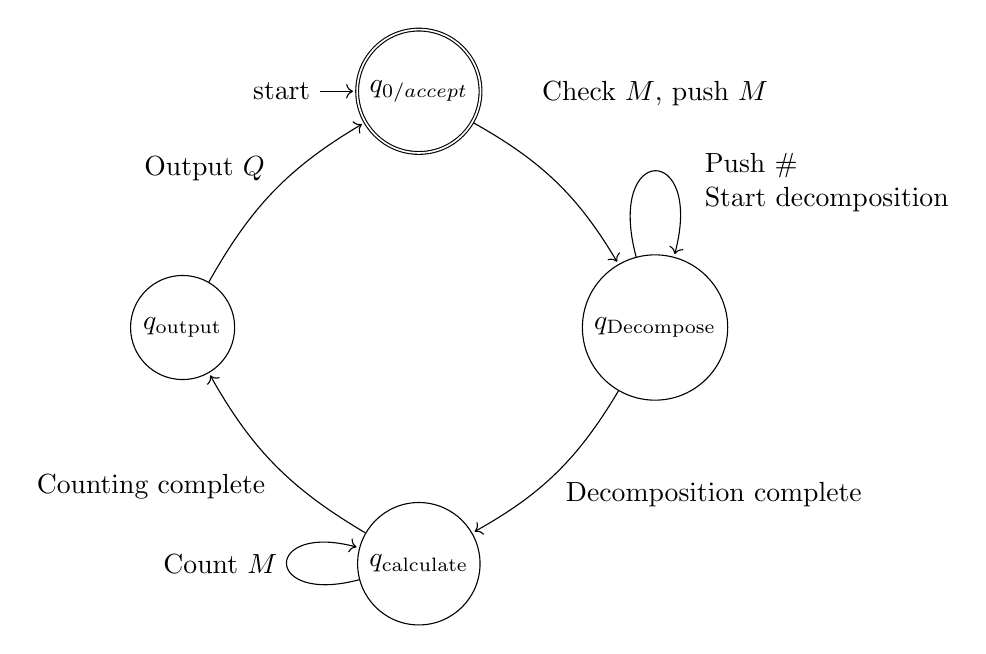
\begin{tikzpicture}[
    shorten >=1pt,
    auto,
    node distance=3cm,
    every state/.style={minimum size=1cm}
]
    % Arrange four states in a circle:
    % q_{0/accept} (merged start and accept) at 90°,
    % q_decompose at 0°,
    % q_calculate at 270°,
    % q_output at 180°.
    \node[state, initial, accepting] (q0) at (90:3cm) {$q_{0/accept}$};
    \node[state] (q1) at (0:3cm) {$q_{\text{Decompose}}$};
    \node[state] (q2) at (270:3cm) {$q_{\text{calculate}}$};
    \node[state] (q3) at (180:3cm) {$q_{\text{output}}$};
    
    \path[->]
        (q0) edge[bend left=15] node[right=50pt, align=left] {Push \(\#\)\\Start decomposition} (q1)
        (q1) edge[loop above] node[above=20pt, align=center] {Check \(M\), push \(M\)} (q1)
        (q1) edge[bend left=15] node[below right, align=center] {Decomposition complete} (q2)
        (q2) edge[loop left] node[left, align=center] {Count \(M\)} (q2)
        (q2) edge[bend left=15] node[below left, align=center] {Counting complete} (q3)
        (q3) edge[bend left=15] node[above left, align=center] {Output \(Q\)} (q0);
\end{tikzpicture}
\end{center}

\subsubsection*{Example Execution}
\textbf{Problem:} Divide 56 items by groups of 8 using the inverse distributive property.
\begin{enumerate}
    \item \textbf{Start:}  
    \begin{itemize}
        \item Stack: \(\#\)
    \end{itemize}
    \item \textbf{Decompose:}  
    \begin{itemize}
        \item 56 can be decomposed as \(8 \times 7\).  
        \item Push 7 multiples of 8 onto the stack.
    \end{itemize}
    \item \textbf{Calculate Quotient:}  
    \begin{itemize}
        \item Count the 7 occurrences of \(M\).
        \item Push \(Q = 7\) onto the stack.
    \end{itemize}
    \item \textbf{Output:}  
    \begin{itemize}
        \item The automaton outputs \(7\), meaning 7 groups of 8.
    \end{itemize}
\end{enumerate}

\subsubsection*{Recursive Handling of Decomposition}
The automaton recursively checks for the largest multiple \(M\) that fits into the remaining total, ensuring an efficient decomposition and accurate quotient calculation.


\subsubsection*{HTML Implementation}
\lstinputlisting[style=htmlStyle, language=html]{./new_html/SMR_DIV_IDP.html}

\printbibliography
\end{document}